\documentclass[1p]{elsarticle_modified}
%\bibliographystyle{elsarticle-num}

%\usepackage[colorlinks]{hyperref}
%\usepackage{abbrmath_seonhwa} %\Abb, \Ascr, \Acal ,\Abf, \Afrak
\usepackage{amsfonts}
\usepackage{amssymb}
\usepackage{amsmath}
\usepackage{amsthm}
\usepackage{scalefnt}
\usepackage{amsbsy}
\usepackage{kotex}
\usepackage{caption}
\usepackage{subfig}
\usepackage{color}
\usepackage{graphicx}
\usepackage{xcolor} %% white, black, red, green, blue, cyan, magenta, yellow
\usepackage{float}
\usepackage{setspace}
\usepackage{hyperref}

\usepackage{tikz}
\usetikzlibrary{arrows}

\usepackage{multirow}
\usepackage{array} % fixed length table
\usepackage{hhline}

%%%%%%%%%%%%%%%%%%%%%
\makeatletter
\renewcommand*\env@matrix[1][\arraystretch]{%
	\edef\arraystretch{#1}%
	\hskip -\arraycolsep
	\let\@ifnextchar\new@ifnextchar
	\array{*\c@MaxMatrixCols c}}
\makeatother %https://tex.stackexchange.com/questions/14071/how-can-i-increase-the-line-spacing-in-a-matrix
%%%%%%%%%%%%%%%

\usepackage[normalem]{ulem}

\newcommand{\msout}[1]{\ifmmode\text{\sout{\ensuremath{#1}}}\else\sout{#1}\fi}
%SOURCE: \msout is \stkout macro in https://tex.stackexchange.com/questions/20609/strikeout-in-math-mode

\newcommand{\cancel}[1]{
	\ifmmode
	{\color{red}\msout{#1}}
	\else
	{\color{red}\sout{#1}}
	\fi
}

\newcommand{\add}[1]{
	{\color{blue}\uwave{#1}}
}

\newcommand{\replace}[2]{
	\ifmmode
	{\color{red}\msout{#1}}{\color{blue}\uwave{#2}}
	\else
	{\color{red}\sout{#1}}{\color{blue}\uwave{#2}}
	\fi
}

\newcommand{\Sol}{\mathcal{S}} %segment
\newcommand{\D}{D} %diagram
\newcommand{\A}{\mathcal{A}} %arc


%%%%%%%%%%%%%%%%%%%%%%%%%%%%%5 test

\def\sl{\operatorname{\textup{SL}}(2,\Cbb)}
\def\psl{\operatorname{\textup{PSL}}(2,\Cbb)}
\def\quan{\mkern 1mu \triangleright \mkern 1mu}

\theoremstyle{definition}
\newtheorem{thm}{Theorem}[section]
\newtheorem{prop}[thm]{Proposition}
\newtheorem{lem}[thm]{Lemma}
\newtheorem{ques}[thm]{Question}
\newtheorem{cor}[thm]{Corollary}
\newtheorem{defn}[thm]{Definition}
\newtheorem{exam}[thm]{Example}
\newtheorem{rmk}[thm]{Remark}
\newtheorem{alg}[thm]{Algorithm}

\newcommand{\I}{\sqrt{-1}}
\begin{document}

%\begin{frontmatter}
%
%\title{Boundary parabolic representations of knots up to 8 crossings}
%
%%% Group authors per affiliation:
%\author{Yunhi Cho} 
%\address{Department of Mathematics, University of Seoul, Seoul, Korea}
%\ead{yhcho@uos.ac.kr}
%
%
%\author{Seonhwa Kim} %\fnref{s_kim}}
%\address{Center for Geometry and Physics, Institute for Basic Science, Pohang, 37673, Korea}
%\ead{ryeona17@ibs.re.kr}
%
%\author{Hyuk Kim}
%\address{Department of Mathematical Sciences, Seoul National University, Seoul 08826, Korea}
%\ead{hyukkim@snu.ac.kr}
%
%\author{Seokbeom Yoon}
%\address{Department of Mathematical Sciences, Seoul National University, Seoul, 08826,  Korea}
%\ead{sbyoon15@snu.ac.kr}
%
%\begin{abstract}
%We find all boundary parabolic representation of knots up to 8 crossings.
%
%\end{abstract}
%\begin{keyword}
%    \MSC[2010] 57M25 
%\end{keyword}
%
%\end{frontmatter}

%\linenumbers
%\tableofcontents
%
\newcommand\colored[1]{\textcolor{white}{\rule[-0.35ex]{0.8em}{1.4ex}}\kern-0.8em\color{red} #1}%
%\newcommand\colored[1]{\textcolor{white}{ #1}\kern-2.17ex	\textcolor{white}{ #1}\kern-1.81ex	\textcolor{white}{ #1}\kern-2.15ex\color{red}#1	}

{\Large $\underline{12a_{1104}~(K12a_{1104})}$}

\setlength{\tabcolsep}{10pt}
\renewcommand{\arraystretch}{1.6}
\vspace{1cm}\begin{tabular}{m{100pt}>{\centering\arraybackslash}m{274pt}}
\multirow{5}{120pt}{
	\centering
	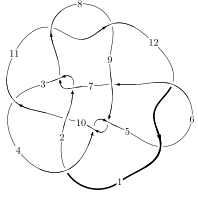
\includegraphics[width=112pt]{../../../GIT/diagram.site/Diagrams/png/1905_12a_1104.png}\\
\ \ \ A knot diagram\footnotemark}&
\allowdisplaybreaks
\textbf{Linearized knot diagam} \\
\cline{2-2}
 &
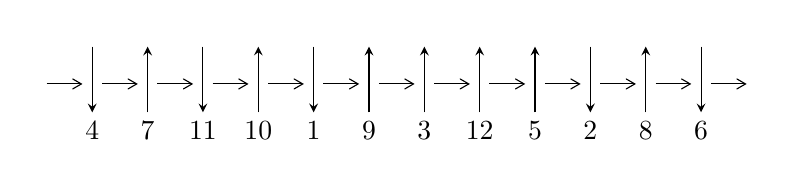
\begin{tikzpicture}[x=20pt, y=17pt]
	% nodes
	\node (C0) at (0, 0) {};
	\node (C1) at (1, 0) {};
	\node (C1U) at (1, +1) {};
	\node (C1D) at (1, -1) {4};

	\node (C2) at (2, 0) {};
	\node (C2U) at (2, +1) {};
	\node (C2D) at (2, -1) {7};

	\node (C3) at (3, 0) {};
	\node (C3U) at (3, +1) {};
	\node (C3D) at (3, -1) {11};

	\node (C4) at (4, 0) {};
	\node (C4U) at (4, +1) {};
	\node (C4D) at (4, -1) {10};

	\node (C5) at (5, 0) {};
	\node (C5U) at (5, +1) {};
	\node (C5D) at (5, -1) {1};

	\node (C6) at (6, 0) {};
	\node (C6U) at (6, +1) {};
	\node (C6D) at (6, -1) {9};

	\node (C7) at (7, 0) {};
	\node (C7U) at (7, +1) {};
	\node (C7D) at (7, -1) {3};

	\node (C8) at (8, 0) {};
	\node (C8U) at (8, +1) {};
	\node (C8D) at (8, -1) {12};

	\node (C9) at (9, 0) {};
	\node (C9U) at (9, +1) {};
	\node (C9D) at (9, -1) {5};

	\node (C10) at (10, 0) {};
	\node (C10U) at (10, +1) {};
	\node (C10D) at (10, -1) {2};

	\node (C11) at (11, 0) {};
	\node (C11U) at (11, +1) {};
	\node (C11D) at (11, -1) {8};

	\node (C12) at (12, 0) {};
	\node (C12U) at (12, +1) {};
	\node (C12D) at (12, -1) {6};
	\node (C13) at (13, 0) {};

	% arrows
	\draw[->,>={angle 60}]
	(C0) edge (C1) (C1) edge (C2) (C2) edge (C3) (C3) edge (C4) (C4) edge (C5) (C5) edge (C6) (C6) edge (C7) (C7) edge (C8) (C8) edge (C9) (C9) edge (C10) (C10) edge (C11) (C11) edge (C12) (C12) edge (C13) ;	\draw[->,>=stealth]
	(C1U) edge (C1D) (C2D) edge (C2U) (C3U) edge (C3D) (C4D) edge (C4U) (C5U) edge (C5D) (C6D) edge (C6U) (C7D) edge (C7U) (C8D) edge (C8U) (C9D) edge (C9U) (C10U) edge (C10D) (C11D) edge (C11U) (C12U) edge (C12D) ;
	\end{tikzpicture} \\
\hhline{~~} \\& 
\textbf{Solving Sequence} \\ \cline{2-2} 
 &
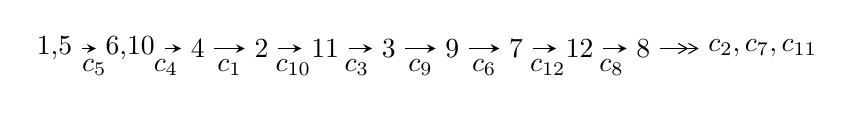
\begin{tikzpicture}[x=23pt, y=7pt]
	% node
	\node (A0) at (-1/8, 0) {1,5};
	\node (A1) at (17/16, 0) {6,10};
	\node (A2) at (17/8, 0) {4};
	\node (A3) at (25/8, 0) {2};
	\node (A4) at (33/8, 0) {11};
	\node (A5) at (41/8, 0) {3};
	\node (A6) at (49/8, 0) {9};
	\node (A7) at (57/8, 0) {7};
	\node (A8) at (65/8, 0) {12};
	\node (A9) at (73/8, 0) {8};
	\node (C1) at (1/2, -1) {$c_{5}$};
	\node (C2) at (13/8, -1) {$c_{4}$};
	\node (C3) at (21/8, -1) {$c_{1}$};
	\node (C4) at (29/8, -1) {$c_{10}$};
	\node (C5) at (37/8, -1) {$c_{3}$};
	\node (C6) at (45/8, -1) {$c_{9}$};
	\node (C7) at (53/8, -1) {$c_{6}$};
	\node (C8) at (61/8, -1) {$c_{12}$};
	\node (C9) at (69/8, -1) {$c_{8}$};
	\node (A10) at (11, 0) {$c_{2},c_{7},c_{11}$};

	% edge
	\draw[->,>=stealth]	
	(A0) edge (A1) (A1) edge (A2) (A2) edge (A3) (A3) edge (A4) (A4) edge (A5) (A5) edge (A6) (A6) edge (A7) (A7) edge (A8) (A8) edge (A9) ;
	\draw[->>,>={angle 60}]	
	(A9) edge (A10);
\end{tikzpicture} \\ 

\end{tabular} \\

\footnotetext{
The image of knot diagram is generated by the software ``\textbf{Draw programme}" developed by Andrew Bartholomew(\url{http://www.layer8.co.uk/maths/draw/index.htm\#Running-draw}), where we modified some parts for our purpose(\url{https://github.com/CATsTAILs/LinksPainter}).
}\phantom \\ \newline 
\centering \textbf{Ideals for irreducible components\footnotemark of $X_{\text{par}}$} 
 
\begin{align*}
I^u_{1}&=\langle 
3.05525\times10^{662} u^{141}+5.78982\times10^{662} u^{140}+\cdots+3.78187\times10^{663} b+1.21271\times10^{664},\\
\phantom{I^u_{1}}&\phantom{= \langle  }-7.67090\times10^{664} u^{141}-2.82754\times10^{665} u^{140}+\cdots+3.89533\times10^{665} a+4.28713\times10^{667},\\
\phantom{I^u_{1}}&\phantom{= \langle  }u^{142}+2 u^{141}+\cdots+4010 u-412\rangle \\
I^u_{2}&=\langle 
7.97745\times10^{22} u^{34}-4.52888\times10^{22} u^{33}+\cdots+1.96845\times10^{23} b+5.61550\times10^{23},\\
\phantom{I^u_{2}}&\phantom{= \langle  }-2.95746\times10^{23} u^{34}+7.02784\times10^{23} u^{33}+\cdots+1.37791\times10^{24} a+1.72399\times10^{25},\;u^{35}- u^{34}+\cdots-35 u+7\rangle \\
\\
\end{align*}
\raggedright * 2 irreducible components of $\dim_{\mathbb{C}}=0$, with total 177 representations.\\
\footnotetext{All coefficients of polynomials are rational numbers. But the coefficients are sometimes approximated in decimal forms when there is not enough margin.}
\newpage
\renewcommand{\arraystretch}{1}
\centering \section*{I. $I^u_{1}= \langle 3.06\times10^{662} u^{141}+5.79\times10^{662} u^{140}+\cdots+3.78\times10^{663} b+1.21\times10^{664},\;-7.67\times10^{664} u^{141}-2.83\times10^{665} u^{140}+\cdots+3.90\times10^{665} a+4.29\times10^{667},\;u^{142}+2 u^{141}+\cdots+4010 u-412 \rangle$}
\flushleft \textbf{(i) Arc colorings}\\
\begin{tabular}{m{7pt} m{180pt} m{7pt} m{180pt} }
\flushright $a_{1}=$&$\begin{pmatrix}0\\u\end{pmatrix}$ \\
\flushright $a_{5}=$&$\begin{pmatrix}1\\0\end{pmatrix}$ \\
\flushright $a_{6}=$&$\begin{pmatrix}1\\u^2\end{pmatrix}$ \\
\flushright $a_{10}=$&$\begin{pmatrix}0.196926 u^{141}+0.725879 u^{140}+\cdots+980.804 u-110.058\\-0.0807868 u^{141}-0.153094 u^{140}+\cdots+67.5667 u-3.20663\end{pmatrix}$ \\
\flushright $a_{4}=$&$\begin{pmatrix}0.270305 u^{141}+0.437638 u^{140}+\cdots-472.743 u+39.6051\\0.0201043 u^{141}+0.170811 u^{140}+\cdots+490.447 u-49.5599\end{pmatrix}$ \\
\flushright $a_{2}=$&$\begin{pmatrix}-0.948288 u^{141}-2.06709 u^{140}+\cdots-90.6345 u+42.4985\\0.200573 u^{141}+0.194482 u^{140}+\cdots-637.339 u+59.0464\end{pmatrix}$ \\
\flushright $a_{11}=$&$\begin{pmatrix}-0.370759 u^{141}-1.19107 u^{140}+\cdots-1276.76 u+142.692\\0.125993 u^{141}+0.216255 u^{140}+\cdots-120.213 u+8.27814\end{pmatrix}$ \\
\flushright $a_{3}=$&$\begin{pmatrix}-0.0807668 u^{141}+1.02275 u^{140}+\cdots+3929.60 u-399.103\\-0.385378 u^{141}-0.719289 u^{140}+\cdots+354.159 u-22.9459\end{pmatrix}$ \\
\flushright $a_{9}=$&$\begin{pmatrix}0.277712 u^{141}+0.878973 u^{140}+\cdots+913.237 u-106.852\\-0.0807868 u^{141}-0.153094 u^{140}+\cdots+67.5667 u-3.20663\end{pmatrix}$ \\
\flushright $a_{7}=$&$\begin{pmatrix}0.251669 u^{141}+1.79219 u^{140}+\cdots+4201.27 u-438.189\\-0.327363 u^{141}-0.543234 u^{140}+\cdots+549.269 u-46.6727\end{pmatrix}$ \\
\flushright $a_{12}=$&$\begin{pmatrix}u\\u^3+u\end{pmatrix}$ \\
\flushright $a_{8}=$&$\begin{pmatrix}0.219032 u^{141}+0.875317 u^{140}+\cdots+1330.79 u-147.900\\-0.0612681 u^{141}-0.127746 u^{140}+\cdots+4.98676 u+2.59114\end{pmatrix}$\\&\end{tabular}
\flushleft \textbf{(ii) Obstruction class $= -1$}\\~\\
\flushleft \textbf{(iii) Cusp Shapes $= 0.0831535 u^{141}-1.45840 u^{140}+\cdots-5560.47 u+578.071$}\\~\\
\newpage\renewcommand{\arraystretch}{1}
\flushleft \textbf{(iv) u-Polynomials at the component}\newline \\
\begin{tabular}{m{50pt}|m{274pt}}
Crossings & \hspace{64pt}u-Polynomials at each crossing \\
\hline $$\begin{aligned}c_{1}\end{aligned}$$&$\begin{aligned}
&u^{142}-16 u^{141}+\cdots+7169 u-211
\end{aligned}$\\
\hline $$\begin{aligned}c_{2},c_{7}\end{aligned}$$&$\begin{aligned}
&u^{142}+u^{141}+\cdots-341251 u+204397
\end{aligned}$\\
\hline $$\begin{aligned}c_{3}\end{aligned}$$&$\begin{aligned}
&u^{142}+32 u^{140}+\cdots+1208588206 u-60612292
\end{aligned}$\\
\hline $$\begin{aligned}c_{4},c_{9}\end{aligned}$$&$\begin{aligned}
&u^{142}-2 u^{141}+\cdots-8812 u-1699
\end{aligned}$\\
\hline $$\begin{aligned}c_{5},c_{12}\end{aligned}$$&$\begin{aligned}
&u^{142}+2 u^{141}+\cdots+4010 u-412
\end{aligned}$\\
\hline $$\begin{aligned}c_{6}\end{aligned}$$&$\begin{aligned}
&u^{142}+16 u^{141}+\cdots-112963913 u-5370727
\end{aligned}$\\
\hline $$\begin{aligned}c_{8},c_{11}\end{aligned}$$&$\begin{aligned}
&u^{142}-4 u^{141}+\cdots-354 u+3629
\end{aligned}$\\
\hline $$\begin{aligned}c_{10}\end{aligned}$$&$\begin{aligned}
&u^{142}+5 u^{141}+\cdots-3890 u-487
\end{aligned}$\\
\hline
\end{tabular}\\~\\
\newpage\renewcommand{\arraystretch}{1}
\flushleft \textbf{(v) Riley Polynomials at the component}\newline \\
\begin{tabular}{m{50pt}|m{274pt}}
Crossings & \hspace{64pt}Riley Polynomials at each crossing \\
\hline $$\begin{aligned}c_{1}\end{aligned}$$&$\begin{aligned}
&y^{142}+10 y^{141}+\cdots+948631 y+44521
\end{aligned}$\\
\hline $$\begin{aligned}c_{2},c_{7}\end{aligned}$$&$\begin{aligned}
&y^{142}-93 y^{141}+\cdots-815359170921 y+41778133609
\end{aligned}$\\
\hline $$\begin{aligned}c_{3}\end{aligned}$$&$\begin{aligned}
&y^{142}+64 y^{141}+\cdots-23240511541676972 y+3673849941493264
\end{aligned}$\\
\hline $$\begin{aligned}c_{4},c_{9}\end{aligned}$$&$\begin{aligned}
&y^{142}+92 y^{141}+\cdots+27075016 y+2886601
\end{aligned}$\\
\hline $$\begin{aligned}c_{5},c_{12}\end{aligned}$$&$\begin{aligned}
&y^{142}+108 y^{141}+\cdots-1067644 y+169744
\end{aligned}$\\
\hline $$\begin{aligned}c_{6}\end{aligned}$$&$\begin{aligned}
&y^{142}-44 y^{141}+\cdots-1340943864837187 y+28844708508529
\end{aligned}$\\
\hline $$\begin{aligned}c_{8},c_{11}\end{aligned}$$&$\begin{aligned}
&y^{142}-124 y^{141}+\cdots-681165230 y+13169641
\end{aligned}$\\
\hline $$\begin{aligned}c_{10}\end{aligned}$$&$\begin{aligned}
&y^{142}-31 y^{141}+\cdots-29207374 y+237169
\end{aligned}$\\
\hline
\end{tabular}\\~\\
\newpage\flushleft \textbf{(vi) Complex Volumes and Cusp Shapes}
$$\begin{array}{c|c|c}  
\text{Solutions to }I^u_{1}& \I (\text{vol} + \sqrt{-1}CS) & \text{Cusp shape}\\
 \hline 
\begin{aligned}
u &= -0.984844 + 0.100509 I \\
a &= -0.07674 + 1.48482 I \\
b &= \phantom{-}0.235660 + 1.217130 I\end{aligned}
 & -2.98013 + 2.73323 I & \phantom{-0.000000 } 0 \\ \hline\begin{aligned}
u &= -0.984844 - 0.100509 I \\
a &= -0.07674 - 1.48482 I \\
b &= \phantom{-}0.235660 - 1.217130 I\end{aligned}
 & -2.98013 - 2.73323 I & \phantom{-0.000000 } 0 \\ \hline\begin{aligned}
u &= -0.837549 + 0.516655 I \\
a &= \phantom{-}0.304621 - 0.437831 I \\
b &= \phantom{-}0.396604 + 0.087733 I\end{aligned}
 & \phantom{-}1.99869 + 3.00411 I & \phantom{-0.000000 } 0 \\ \hline\begin{aligned}
u &= -0.837549 - 0.516655 I \\
a &= \phantom{-}0.304621 + 0.437831 I \\
b &= \phantom{-}0.396604 - 0.087733 I\end{aligned}
 & \phantom{-}1.99869 - 3.00411 I & \phantom{-0.000000 } 0 \\ \hline\begin{aligned}
u &= \phantom{-}0.159651 + 0.969202 I \\
a &= \phantom{-}0.915581 + 0.848278 I \\
b &= -0.87280 + 1.43805 I\end{aligned}
 & \phantom{-}0.39178 - 3.45919 I & \phantom{-0.000000 } 0 \\ \hline\begin{aligned}
u &= \phantom{-}0.159651 - 0.969202 I \\
a &= \phantom{-}0.915581 - 0.848278 I \\
b &= -0.87280 - 1.43805 I\end{aligned}
 & \phantom{-}0.39178 + 3.45919 I & \phantom{-0.000000 } 0 \\ \hline\begin{aligned}
u &= \phantom{-}0.020124 + 1.038610 I \\
a &= \phantom{-}0.80847 + 1.75248 I \\
b &= -0.27819 + 1.45207 I\end{aligned}
 & \phantom{-}1.59131 - 2.90380 I & \phantom{-0.000000 } 0 \\ \hline\begin{aligned}
u &= \phantom{-}0.020124 - 1.038610 I \\
a &= \phantom{-}0.80847 - 1.75248 I \\
b &= -0.27819 - 1.45207 I\end{aligned}
 & \phantom{-}1.59131 + 2.90380 I & \phantom{-0.000000 } 0 \\ \hline\begin{aligned}
u &= \phantom{-}0.125882 + 0.946218 I \\
a &= -2.49078 - 0.00646 I \\
b &= \phantom{-}0.005305 + 0.800647 I\end{aligned}
 & \phantom{-}6.81084 - 7.72246 I & \phantom{-0.000000 } 0 \\ \hline\begin{aligned}
u &= \phantom{-}0.125882 - 0.946218 I \\
a &= -2.49078 + 0.00646 I \\
b &= \phantom{-}0.005305 - 0.800647 I\end{aligned}
 & \phantom{-}6.81084 + 7.72246 I & \phantom{-0.000000 } 0\\
 \hline 
 \end{array}$$\newpage$$\begin{array}{c|c|c}  
\text{Solutions to }I^u_{1}& \I (\text{vol} + \sqrt{-1}CS) & \text{Cusp shape}\\
 \hline 
\begin{aligned}
u &= \phantom{-}0.402138 + 0.969068 I \\
a &= -1.52524 - 0.74812 I \\
b &= \phantom{-}0.041875 - 1.002700 I\end{aligned}
 & -2.82256 - 0.10966 I & \phantom{-0.000000 } 0 \\ \hline\begin{aligned}
u &= \phantom{-}0.402138 - 0.969068 I \\
a &= -1.52524 + 0.74812 I \\
b &= \phantom{-}0.041875 + 1.002700 I\end{aligned}
 & -2.82256 + 0.10966 I & \phantom{-0.000000 } 0 \\ \hline\begin{aligned}
u &= \phantom{-}1.027770 + 0.228022 I \\
a &= -0.50653 - 1.54130 I \\
b &= -0.285803 - 1.225280 I\end{aligned}
 & -5.10559 + 3.34538 I & \phantom{-0.000000 } 0 \\ \hline\begin{aligned}
u &= \phantom{-}1.027770 - 0.228022 I \\
a &= -0.50653 + 1.54130 I \\
b &= -0.285803 + 1.225280 I\end{aligned}
 & -5.10559 - 3.34538 I & \phantom{-0.000000 } 0 \\ \hline\begin{aligned}
u &= -0.353010 + 0.865129 I \\
a &= -1.007260 + 0.972687 I \\
b &= \phantom{-}0.97052 + 1.15419 I\end{aligned}
 & \phantom{-}1.40884 + 5.10516 I & \phantom{-0.000000 } 0 \\ \hline\begin{aligned}
u &= -0.353010 - 0.865129 I \\
a &= -1.007260 - 0.972687 I \\
b &= \phantom{-}0.97052 - 1.15419 I\end{aligned}
 & \phantom{-}1.40884 - 5.10516 I & \phantom{-0.000000 } 0 \\ \hline\begin{aligned}
u &= \phantom{-}0.491061 + 0.793014 I \\
a &= \phantom{-}0.751971 + 0.457743 I \\
b &= \phantom{-}0.288084 + 1.363560 I\end{aligned}
 & \phantom{-}0.381433 + 1.036770 I & \phantom{-0.000000 } 0 \\ \hline\begin{aligned}
u &= \phantom{-}0.491061 - 0.793014 I \\
a &= \phantom{-}0.751971 - 0.457743 I \\
b &= \phantom{-}0.288084 - 1.363560 I\end{aligned}
 & \phantom{-}0.381433 - 1.036770 I & \phantom{-0.000000 } 0 \\ \hline\begin{aligned}
u &= -1.059720 + 0.172686 I \\
a &= \phantom{-}0.45796 - 1.39635 I \\
b &= \phantom{-}0.392651 - 1.259040 I\end{aligned}
 & -2.54300 - 7.72600 I & \phantom{-0.000000 } 0 \\ \hline\begin{aligned}
u &= -1.059720 - 0.172686 I \\
a &= \phantom{-}0.45796 + 1.39635 I \\
b &= \phantom{-}0.392651 + 1.259040 I\end{aligned}
 & -2.54300 + 7.72600 I & \phantom{-0.000000 } 0\\
 \hline 
 \end{array}$$\newpage$$\begin{array}{c|c|c}  
\text{Solutions to }I^u_{1}& \I (\text{vol} + \sqrt{-1}CS) & \text{Cusp shape}\\
 \hline 
\begin{aligned}
u &= \phantom{-}0.736330 + 0.799939 I \\
a &= \phantom{-}0.61366 + 2.48024 I \\
b &= -0.101180 + 1.181560 I\end{aligned}
 & -0.73713 - 2.79109 I & \phantom{-0.000000 } 0 \\ \hline\begin{aligned}
u &= \phantom{-}0.736330 - 0.799939 I \\
a &= \phantom{-}0.61366 - 2.48024 I \\
b &= -0.101180 - 1.181560 I\end{aligned}
 & -0.73713 + 2.79109 I & \phantom{-0.000000 } 0 \\ \hline\begin{aligned}
u &= \phantom{-}0.500442 + 0.979743 I \\
a &= \phantom{-}0.885614 + 1.054560 I \\
b &= -0.721025 + 0.688788 I\end{aligned}
 & \phantom{-}3.36940 - 4.37250 I & \phantom{-0.000000 } 0 \\ \hline\begin{aligned}
u &= \phantom{-}0.500442 - 0.979743 I \\
a &= \phantom{-}0.885614 - 1.054560 I \\
b &= -0.721025 - 0.688788 I\end{aligned}
 & \phantom{-}3.36940 + 4.37250 I & \phantom{-0.000000 } 0 \\ \hline\begin{aligned}
u &= \phantom{-}1.022420 + 0.407245 I \\
a &= -0.088640 - 0.742762 I \\
b &= -0.355072 - 0.312958 I\end{aligned}
 & \phantom{-}6.81363 + 3.28356 I & \phantom{-0.000000 } 0 \\ \hline\begin{aligned}
u &= \phantom{-}1.022420 - 0.407245 I \\
a &= -0.088640 + 0.742762 I \\
b &= -0.355072 + 0.312958 I\end{aligned}
 & \phantom{-}6.81363 - 3.28356 I & \phantom{-0.000000 } 0 \\ \hline\begin{aligned}
u &= \phantom{-}0.012099 + 1.100730 I \\
a &= -2.03119 + 1.18051 I \\
b &= \phantom{-}0.438524 + 1.095800 I\end{aligned}
 & \phantom{-}7.67363 + 7.16298 I & \phantom{-0.000000 } 0 \\ \hline\begin{aligned}
u &= \phantom{-}0.012099 - 1.100730 I \\
a &= -2.03119 - 1.18051 I \\
b &= \phantom{-}0.438524 - 1.095800 I\end{aligned}
 & \phantom{-}7.67363 - 7.16298 I & \phantom{-0.000000 } 0 \\ \hline\begin{aligned}
u &= -0.030761 + 1.114620 I \\
a &= -0.102542 + 0.237721 I \\
b &= \phantom{-}0.528914 + 0.804634 I\end{aligned}
 & \phantom{-}1.43451 + 2.04369 I & \phantom{-0.000000 } 0 \\ \hline\begin{aligned}
u &= -0.030761 - 1.114620 I \\
a &= -0.102542 - 0.237721 I \\
b &= \phantom{-}0.528914 - 0.804634 I\end{aligned}
 & \phantom{-}1.43451 - 2.04369 I & \phantom{-0.000000 } 0\\
 \hline 
 \end{array}$$\newpage$$\begin{array}{c|c|c}  
\text{Solutions to }I^u_{1}& \I (\text{vol} + \sqrt{-1}CS) & \text{Cusp shape}\\
 \hline 
\begin{aligned}
u &= -0.589533 + 0.655355 I \\
a &= -0.720172 + 0.493276 I \\
b &= -0.484815 + 1.284090 I\end{aligned}
 & \phantom{-}0.92179 - 1.20069 I & \phantom{-0.000000 } 0 \\ \hline\begin{aligned}
u &= -0.589533 - 0.655355 I \\
a &= -0.720172 - 0.493276 I \\
b &= -0.484815 - 1.284090 I\end{aligned}
 & \phantom{-}0.92179 + 1.20069 I & \phantom{-0.000000 } 0 \\ \hline\begin{aligned}
u &= \phantom{-}0.201197 + 1.100460 I \\
a &= \phantom{-}0.165503 + 0.117893 I \\
b &= -1.56098 - 0.16282 I\end{aligned}
 & \phantom{-}4.68480 - 6.08536 I & \phantom{-0.000000 } 0 \\ \hline\begin{aligned}
u &= \phantom{-}0.201197 - 1.100460 I \\
a &= \phantom{-}0.165503 - 0.117893 I \\
b &= -1.56098 + 0.16282 I\end{aligned}
 & \phantom{-}4.68480 + 6.08536 I & \phantom{-0.000000 } 0 \\ \hline\begin{aligned}
u &= \phantom{-}0.051461 + 1.119110 I \\
a &= \phantom{-}0.662635 - 0.747892 I \\
b &= -0.683630 - 1.158830 I\end{aligned}
 & \phantom{-}4.29429 - 0.88376 I & \phantom{-0.000000 } 0 \\ \hline\begin{aligned}
u &= \phantom{-}0.051461 - 1.119110 I \\
a &= \phantom{-}0.662635 + 0.747892 I \\
b &= -0.683630 + 1.158830 I\end{aligned}
 & \phantom{-}4.29429 + 0.88376 I & \phantom{-0.000000 } 0 \\ \hline\begin{aligned}
u &= -0.351825 + 1.069190 I \\
a &= \phantom{-}0.159352 + 0.204363 I \\
b &= -0.063648 + 0.484219 I\end{aligned}
 & \phantom{-}1.12198 + 2.22225 I & \phantom{-0.000000 } 0 \\ \hline\begin{aligned}
u &= -0.351825 - 1.069190 I \\
a &= \phantom{-}0.159352 - 0.204363 I \\
b &= -0.063648 - 0.484219 I\end{aligned}
 & \phantom{-}1.12198 - 2.22225 I & \phantom{-0.000000 } 0 \\ \hline\begin{aligned}
u &= -0.033328 + 0.869696 I \\
a &= \phantom{-}1.216540 - 0.619281 I \\
b &= \phantom{-}0.074886 + 0.926726 I\end{aligned}
 & \phantom{-}1.00387 + 2.75697 I & \phantom{-0.000000 } 0 \\ \hline\begin{aligned}
u &= -0.033328 - 0.869696 I \\
a &= \phantom{-}1.216540 + 0.619281 I \\
b &= \phantom{-}0.074886 - 0.926726 I\end{aligned}
 & \phantom{-}1.00387 - 2.75697 I & \phantom{-0.000000 } 0\\
 \hline 
 \end{array}$$\newpage$$\begin{array}{c|c|c}  
\text{Solutions to }I^u_{1}& \I (\text{vol} + \sqrt{-1}CS) & \text{Cusp shape}\\
 \hline 
\begin{aligned}
u &= -0.063929 + 1.128370 I \\
a &= -0.325405 - 0.507623 I \\
b &= \phantom{-}1.15997 - 1.64226 I\end{aligned}
 & \phantom{-}7.03090 + 4.88414 I & \phantom{-0.000000 } 0 \\ \hline\begin{aligned}
u &= -0.063929 - 1.128370 I \\
a &= -0.325405 + 0.507623 I \\
b &= \phantom{-}1.15997 + 1.64226 I\end{aligned}
 & \phantom{-}7.03090 - 4.88414 I & \phantom{-0.000000 } 0 \\ \hline\begin{aligned}
u &= -0.132830 + 1.141590 I \\
a &= -0.202494 + 0.193407 I \\
b &= \phantom{-}1.212940 + 0.135295 I\end{aligned}
 & \phantom{-}2.50026 + 2.59648 I & \phantom{-0.000000 } 0 \\ \hline\begin{aligned}
u &= -0.132830 - 1.141590 I \\
a &= -0.202494 - 0.193407 I \\
b &= \phantom{-}1.212940 - 0.135295 I\end{aligned}
 & \phantom{-}2.50026 - 2.59648 I & \phantom{-0.000000 } 0 \\ \hline\begin{aligned}
u &= \phantom{-}0.012626 + 1.150960 I \\
a &= -0.73883 - 1.68597 I \\
b &= \phantom{-}0.246263 - 1.003090 I\end{aligned}
 & \phantom{-}8.02783 - 1.44802 I & \phantom{-0.000000 } 0 \\ \hline\begin{aligned}
u &= \phantom{-}0.012626 - 1.150960 I \\
a &= -0.73883 + 1.68597 I \\
b &= \phantom{-}0.246263 + 1.003090 I\end{aligned}
 & \phantom{-}8.02783 + 1.44802 I & \phantom{-0.000000 } 0 \\ \hline\begin{aligned}
u &= \phantom{-}0.811479 + 0.101720 I \\
a &= \phantom{-}0.19077 + 1.84647 I \\
b &= -0.433648 + 1.295380 I\end{aligned}
 & -1.85895 - 4.89496 I & \phantom{-0.000000 } 0 \\ \hline\begin{aligned}
u &= \phantom{-}0.811479 - 0.101720 I \\
a &= \phantom{-}0.19077 - 1.84647 I \\
b &= -0.433648 - 1.295380 I\end{aligned}
 & -1.85895 + 4.89496 I & \phantom{-0.000000 } 0 \\ \hline\begin{aligned}
u &= -0.333376 + 1.150990 I \\
a &= \phantom{-}1.27863 - 1.42598 I \\
b &= -0.468521 - 1.170770 I\end{aligned}
 & \phantom{-}3.92046 + 6.46301 I & \phantom{-0.000000 } 0 \\ \hline\begin{aligned}
u &= -0.333376 - 1.150990 I \\
a &= \phantom{-}1.27863 + 1.42598 I \\
b &= -0.468521 + 1.170770 I\end{aligned}
 & \phantom{-}3.92046 - 6.46301 I & \phantom{-0.000000 } 0\\
 \hline 
 \end{array}$$\newpage$$\begin{array}{c|c|c}  
\text{Solutions to }I^u_{1}& \I (\text{vol} + \sqrt{-1}CS) & \text{Cusp shape}\\
 \hline 
\begin{aligned}
u &= \phantom{-}0.147710 + 1.190750 I \\
a &= \phantom{-}0.473182 - 0.072572 I \\
b &= -1.260080 - 0.431344 I\end{aligned}
 & \phantom{-}4.50046 - 1.69205 I & \phantom{-0.000000 } 0 \\ \hline\begin{aligned}
u &= \phantom{-}0.147710 - 1.190750 I \\
a &= \phantom{-}0.473182 + 0.072572 I \\
b &= -1.260080 + 0.431344 I\end{aligned}
 & \phantom{-}4.50046 + 1.69205 I & \phantom{-0.000000 } 0 \\ \hline\begin{aligned}
u &= \phantom{-}0.729099 + 0.322322 I \\
a &= -0.488169 - 0.632094 I \\
b &= -0.709581 + 0.150857 I\end{aligned}
 & \phantom{-}6.55918 - 8.88010 I & \phantom{-0.000000 } 0 \\ \hline\begin{aligned}
u &= \phantom{-}0.729099 - 0.322322 I \\
a &= -0.488169 + 0.632094 I \\
b &= -0.709581 - 0.150857 I\end{aligned}
 & \phantom{-}6.55918 + 8.88010 I & \phantom{-0.000000 } 0 \\ \hline\begin{aligned}
u &= -0.250296 + 1.177440 I \\
a &= -0.646113 + 0.370855 I \\
b &= \phantom{-}1.019400 - 0.326461 I\end{aligned}
 & \phantom{-}5.75375 + 3.24573 I & \phantom{-0.000000 } 0 \\ \hline\begin{aligned}
u &= -0.250296 - 1.177440 I \\
a &= -0.646113 - 0.370855 I \\
b &= \phantom{-}1.019400 + 0.326461 I\end{aligned}
 & \phantom{-}5.75375 - 3.24573 I & \phantom{-0.000000 } 0 \\ \hline\begin{aligned}
u &= \phantom{-}0.547801 + 1.077520 I \\
a &= \phantom{-}0.256223 + 1.372200 I \\
b &= -0.234284 + 0.867860 I\end{aligned}
 & \phantom{-}3.24949 + 0.44742 I & \phantom{-0.000000 } 0 \\ \hline\begin{aligned}
u &= \phantom{-}0.547801 - 1.077520 I \\
a &= \phantom{-}0.256223 - 1.372200 I \\
b &= -0.234284 - 0.867860 I\end{aligned}
 & \phantom{-}3.24949 - 0.44742 I & \phantom{-0.000000 } 0 \\ \hline\begin{aligned}
u &= -0.506869 + 1.114920 I \\
a &= -0.635883 + 1.006870 I \\
b &= \phantom{-}0.396242 + 1.050570 I\end{aligned}
 & \phantom{-}0.11668 + 2.80990 I & \phantom{-0.000000 } 0 \\ \hline\begin{aligned}
u &= -0.506869 - 1.114920 I \\
a &= -0.635883 - 1.006870 I \\
b &= \phantom{-}0.396242 - 1.050570 I\end{aligned}
 & \phantom{-}0.11668 - 2.80990 I & \phantom{-0.000000 } 0\\
 \hline 
 \end{array}$$\newpage$$\begin{array}{c|c|c}  
\text{Solutions to }I^u_{1}& \I (\text{vol} + \sqrt{-1}CS) & \text{Cusp shape}\\
 \hline 
\begin{aligned}
u &= -0.094898 + 1.232560 I \\
a &= -0.009661 - 0.919156 I \\
b &= \phantom{-}0.12425 - 1.77302 I\end{aligned}
 & \phantom{-}6.64012 - 2.25510 I & \phantom{-0.000000 } 0 \\ \hline\begin{aligned}
u &= -0.094898 - 1.232560 I \\
a &= -0.009661 + 0.919156 I \\
b &= \phantom{-}0.12425 + 1.77302 I\end{aligned}
 & \phantom{-}6.64012 + 2.25510 I & \phantom{-0.000000 } 0 \\ \hline\begin{aligned}
u &= -0.335351 + 1.193370 I \\
a &= \phantom{-}1.226050 - 0.219938 I \\
b &= -0.220502 - 1.042280 I\end{aligned}
 & -0.02084 + 5.39245 I & \phantom{-0.000000 } 0 \\ \hline\begin{aligned}
u &= -0.335351 - 1.193370 I \\
a &= \phantom{-}1.226050 + 0.219938 I \\
b &= -0.220502 + 1.042280 I\end{aligned}
 & -0.02084 - 5.39245 I & \phantom{-0.000000 } 0 \\ \hline\begin{aligned}
u &= -0.747572 + 0.128671 I \\
a &= -0.49664 + 1.50193 I \\
b &= -0.101558 + 1.328870 I\end{aligned}
 & -3.94786 + 1.80337 I & \phantom{-0.000000 } 0 \\ \hline\begin{aligned}
u &= -0.747572 - 0.128671 I \\
a &= -0.49664 - 1.50193 I \\
b &= -0.101558 - 1.328870 I\end{aligned}
 & -3.94786 - 1.80337 I & \phantom{-0.000000 } 0 \\ \hline\begin{aligned}
u &= -0.405635 + 1.175390 I \\
a &= -0.752858 + 0.787150 I \\
b &= \phantom{-}0.54417 + 1.36541 I\end{aligned}
 & -0.78315 + 2.47950 I & \phantom{-0.000000 } 0 \\ \hline\begin{aligned}
u &= -0.405635 - 1.175390 I \\
a &= -0.752858 - 0.787150 I \\
b &= \phantom{-}0.54417 - 1.36541 I\end{aligned}
 & -0.78315 - 2.47950 I & \phantom{-0.000000 } 0 \\ \hline\begin{aligned}
u &= \phantom{-}0.284070 + 1.218590 I \\
a &= \phantom{-}0.832136 + 0.706336 I \\
b &= -0.73081 + 1.40728 I\end{aligned}
 & -0.75549 - 6.15893 I & \phantom{-0.000000 } 0 \\ \hline\begin{aligned}
u &= \phantom{-}0.284070 - 1.218590 I \\
a &= \phantom{-}0.832136 - 0.706336 I \\
b &= -0.73081 - 1.40728 I\end{aligned}
 & -0.75549 + 6.15893 I & \phantom{-0.000000 } 0\\
 \hline 
 \end{array}$$\newpage$$\begin{array}{c|c|c}  
\text{Solutions to }I^u_{1}& \I (\text{vol} + \sqrt{-1}CS) & \text{Cusp shape}\\
 \hline 
\begin{aligned}
u &= \phantom{-}0.133985 + 1.279170 I \\
a &= \phantom{-}0.293297 + 0.419844 I \\
b &= -0.760921 - 0.343237 I\end{aligned}
 & \phantom{-}6.55785 - 1.81776 I & \phantom{-0.000000 } 0 \\ \hline\begin{aligned}
u &= \phantom{-}0.133985 - 1.279170 I \\
a &= \phantom{-}0.293297 - 0.419844 I \\
b &= -0.760921 + 0.343237 I\end{aligned}
 & \phantom{-}6.55785 + 1.81776 I & \phantom{-0.000000 } 0 \\ \hline\begin{aligned}
u &= -0.392859 + 1.232280 I \\
a &= -1.92821 + 0.60627 I \\
b &= \phantom{-}0.153617 + 1.076700 I\end{aligned}
 & \phantom{-}5.53811 + 8.66077 I & \phantom{-0.000000 } 0 \\ \hline\begin{aligned}
u &= -0.392859 - 1.232280 I \\
a &= -1.92821 - 0.60627 I \\
b &= \phantom{-}0.153617 - 1.076700 I\end{aligned}
 & \phantom{-}5.53811 - 8.66077 I & \phantom{-0.000000 } 0 \\ \hline\begin{aligned}
u &= -1.289180 + 0.141154 I \\
a &= -0.11935 - 1.53693 I \\
b &= -0.399278 - 1.265740 I\end{aligned}
 & \phantom{-}2.41747 + 12.94450 I & \phantom{-0.000000 } 0 \\ \hline\begin{aligned}
u &= -1.289180 - 0.141154 I \\
a &= -0.11935 + 1.53693 I \\
b &= -0.399278 + 1.265740 I\end{aligned}
 & \phantom{-}2.41747 - 12.94450 I & \phantom{-0.000000 } 0 \\ \hline\begin{aligned}
u &= -0.677472 + 0.158627 I \\
a &= \phantom{-}1.17293 + 2.48956 I \\
b &= -0.050436 + 1.273870 I\end{aligned}
 & \phantom{-}2.24466 - 4.58437 I & \phantom{-0.000000 } 0 \\ \hline\begin{aligned}
u &= -0.677472 - 0.158627 I \\
a &= \phantom{-}1.17293 - 2.48956 I \\
b &= -0.050436 - 1.273870 I\end{aligned}
 & \phantom{-}2.24466 + 4.58437 I & \phantom{-0.000000 } 0 \\ \hline\begin{aligned}
u &= \phantom{-}0.334793 + 0.602200 I \\
a &= -0.25524 - 2.60301 I \\
b &= \phantom{-}0.161516 - 1.330680 I\end{aligned}
 & -4.17471 - 3.49050 I & \phantom{-0.000000 } 0 \\ \hline\begin{aligned}
u &= \phantom{-}0.334793 - 0.602200 I \\
a &= -0.25524 + 2.60301 I \\
b &= \phantom{-}0.161516 + 1.330680 I\end{aligned}
 & -4.17471 + 3.49050 I & \phantom{-0.000000 } 0\\
 \hline 
 \end{array}$$\newpage$$\begin{array}{c|c|c}  
\text{Solutions to }I^u_{1}& \I (\text{vol} + \sqrt{-1}CS) & \text{Cusp shape}\\
 \hline 
\begin{aligned}
u &= \phantom{-}0.514928 + 1.215670 I \\
a &= -0.81771 - 1.20409 I \\
b &= \phantom{-}0.56891 - 1.36953 I\end{aligned}
 & -1.97519 - 8.74758 I & \phantom{-0.000000 } 0 \\ \hline\begin{aligned}
u &= \phantom{-}0.514928 - 1.215670 I \\
a &= -0.81771 + 1.20409 I \\
b &= \phantom{-}0.56891 + 1.36953 I\end{aligned}
 & -1.97519 + 8.74758 I & \phantom{-0.000000 } 0 \\ \hline\begin{aligned}
u &= -0.641631\phantom{ +0.000000I} \\
a &= -0.361749\phantom{ +0.000000I} \\
b &= -0.945080\phantom{ +0.000000I}\end{aligned}
 & \phantom{-}2.24523\phantom{ +0.000000I} & \phantom{-0.000000 } 0 \\ \hline\begin{aligned}
u &= -0.103611 + 0.633089 I \\
a &= \phantom{-}2.46896 - 1.13103 I \\
b &= \phantom{-}0.084713 - 0.668236 I\end{aligned}
 & \phantom{-}1.71380 - 3.81572 I & \phantom{-0.000000 } 0 \\ \hline\begin{aligned}
u &= -0.103611 - 0.633089 I \\
a &= \phantom{-}2.46896 + 1.13103 I \\
b &= \phantom{-}0.084713 + 0.668236 I\end{aligned}
 & \phantom{-}1.71380 + 3.81572 I & \phantom{-0.000000 } 0 \\ \hline\begin{aligned}
u &= -0.550434 + 1.249550 I \\
a &= \phantom{-}0.782017 - 1.116340 I \\
b &= -0.67922 - 1.37384 I\end{aligned}
 & \phantom{-}0.83467 + 13.38690 I & \phantom{-0.000000 } 0 \\ \hline\begin{aligned}
u &= -0.550434 - 1.249550 I \\
a &= \phantom{-}0.782017 + 1.116340 I \\
b &= -0.67922 + 1.37384 I\end{aligned}
 & \phantom{-}0.83467 - 13.38690 I & \phantom{-0.000000 } 0 \\ \hline\begin{aligned}
u &= -1.304080 + 0.433114 I \\
a &= -0.28455 + 1.44750 I \\
b &= -0.265086 + 0.897059 I\end{aligned}
 & \phantom{-}5.56027 + 0.43931 I & \phantom{-0.000000 } 0 \\ \hline\begin{aligned}
u &= -1.304080 - 0.433114 I \\
a &= -0.28455 - 1.44750 I \\
b &= -0.265086 - 0.897059 I\end{aligned}
 & \phantom{-}5.56027 - 0.43931 I & \phantom{-0.000000 } 0 \\ \hline\begin{aligned}
u &= -0.106693 + 1.374270 I \\
a &= -0.643023 - 0.662664 I \\
b &= \phantom{-}0.635651 + 0.497658 I\end{aligned}
 & \phantom{-}9.58969 - 2.92096 I & \phantom{-0.000000 } 0\\
 \hline 
 \end{array}$$\newpage$$\begin{array}{c|c|c}  
\text{Solutions to }I^u_{1}& \I (\text{vol} + \sqrt{-1}CS) & \text{Cusp shape}\\
 \hline 
\begin{aligned}
u &= -0.106693 - 1.374270 I \\
a &= -0.643023 + 0.662664 I \\
b &= \phantom{-}0.635651 - 0.497658 I\end{aligned}
 & \phantom{-}9.58969 + 2.92096 I & \phantom{-0.000000 } 0 \\ \hline\begin{aligned}
u &= \phantom{-}0.344834 + 1.354110 I \\
a &= -0.151878 - 0.194817 I \\
b &= \phantom{-}1.277670 + 0.012876 I\end{aligned}
 & \phantom{-}11.6455 - 12.7871 I & \phantom{-0.000000 } 0 \\ \hline\begin{aligned}
u &= \phantom{-}0.344834 - 1.354110 I \\
a &= -0.151878 + 0.194817 I \\
b &= \phantom{-}1.277670 - 0.012876 I\end{aligned}
 & \phantom{-}11.6455 + 12.7871 I & \phantom{-0.000000 } 0 \\ \hline\begin{aligned}
u &= \phantom{-}0.186444 + 1.387060 I \\
a &= \phantom{-}0.263370 - 0.425934 I \\
b &= -0.811606 - 0.090491 I\end{aligned}
 & \phantom{-}6.65306 - 1.33256 I & \phantom{-0.000000 } 0 \\ \hline\begin{aligned}
u &= \phantom{-}0.186444 - 1.387060 I \\
a &= \phantom{-}0.263370 + 0.425934 I \\
b &= -0.811606 + 0.090491 I\end{aligned}
 & \phantom{-}6.65306 + 1.33256 I & \phantom{-0.000000 } 0 \\ \hline\begin{aligned}
u &= \phantom{-}0.517473 + 0.289663 I \\
a &= \phantom{-}0.328404 + 0.316082 I \\
b &= \phantom{-}0.613567 + 0.454916 I\end{aligned}
 & \phantom{-}1.84402 + 0.39595 I & \phantom{-0.000000 } 0 \\ \hline\begin{aligned}
u &= \phantom{-}0.517473 - 0.289663 I \\
a &= \phantom{-}0.328404 - 0.316082 I \\
b &= \phantom{-}0.613567 - 0.454916 I\end{aligned}
 & \phantom{-}1.84402 - 0.39595 I & \phantom{-0.000000 } 0 \\ \hline\begin{aligned}
u &= -0.358800 + 1.361140 I \\
a &= -0.004523 - 0.281606 I \\
b &= \phantom{-}0.906616 - 0.581144 I\end{aligned}
 & \phantom{-}11.43760 + 4.96030 I & \phantom{-0.000000 } 0 \\ \hline\begin{aligned}
u &= -0.358800 - 1.361140 I \\
a &= -0.004523 + 0.281606 I \\
b &= \phantom{-}0.906616 + 0.581144 I\end{aligned}
 & \phantom{-}11.43760 - 4.96030 I & \phantom{-0.000000 } 0 \\ \hline\begin{aligned}
u &= \phantom{-}0.388467 + 1.356040 I \\
a &= -1.145520 - 0.799830 I \\
b &= \phantom{-}0.62638 - 1.27303 I\end{aligned}
 & \phantom{-}2.72873 - 9.28905 I & \phantom{-0.000000 } 0\\
 \hline 
 \end{array}$$\newpage$$\begin{array}{c|c|c}  
\text{Solutions to }I^u_{1}& \I (\text{vol} + \sqrt{-1}CS) & \text{Cusp shape}\\
 \hline 
\begin{aligned}
u &= \phantom{-}0.388467 - 1.356040 I \\
a &= -1.145520 + 0.799830 I \\
b &= \phantom{-}0.62638 + 1.27303 I\end{aligned}
 & \phantom{-}2.72873 + 9.28905 I & \phantom{-0.000000 } 0 \\ \hline\begin{aligned}
u &= \phantom{-}0.68750 + 1.23897 I \\
a &= \phantom{-}0.89157 + 1.10859 I \\
b &= -0.130371 + 0.989025 I\end{aligned}
 & -0.03567 - 3.59247 I & \phantom{-0.000000 } 0 \\ \hline\begin{aligned}
u &= \phantom{-}0.68750 - 1.23897 I \\
a &= \phantom{-}0.89157 - 1.10859 I \\
b &= -0.130371 - 0.989025 I\end{aligned}
 & -0.03567 + 3.59247 I & \phantom{-0.000000 } 0 \\ \hline\begin{aligned}
u &= -0.33148 + 1.38849 I \\
a &= \phantom{-}0.158467 - 0.142914 I \\
b &= -1.087720 - 0.069023 I\end{aligned}
 & \phantom{-}7.75860 + 6.98523 I & \phantom{-0.000000 } 0 \\ \hline\begin{aligned}
u &= -0.33148 - 1.38849 I \\
a &= \phantom{-}0.158467 + 0.142914 I \\
b &= -1.087720 + 0.069023 I\end{aligned}
 & \phantom{-}7.75860 - 6.98523 I & \phantom{-0.000000 } 0 \\ \hline\begin{aligned}
u &= -0.44676 + 1.36923 I \\
a &= \phantom{-}0.892811 - 0.809524 I \\
b &= -0.582048 - 1.249040 I\end{aligned}
 & \phantom{-}1.63254 + 7.81762 I & \phantom{-0.000000 } 0 \\ \hline\begin{aligned}
u &= -0.44676 - 1.36923 I \\
a &= \phantom{-}0.892811 + 0.809524 I \\
b &= -0.582048 + 1.249040 I\end{aligned}
 & \phantom{-}1.63254 - 7.81762 I & \phantom{-0.000000 } 0 \\ \hline\begin{aligned}
u &= \phantom{-}0.36967 + 1.42138 I \\
a &= -0.0855022 - 0.0978237 I \\
b &= \phantom{-}0.875379 + 0.154922 I\end{aligned}
 & \phantom{-}12.50620 - 1.51785 I & \phantom{-0.000000 } 0 \\ \hline\begin{aligned}
u &= \phantom{-}0.36967 - 1.42138 I \\
a &= -0.0855022 + 0.0978237 I \\
b &= \phantom{-}0.875379 - 0.154922 I\end{aligned}
 & \phantom{-}12.50620 + 1.51785 I & \phantom{-0.000000 } 0 \\ \hline\begin{aligned}
u &= \phantom{-}1.48953 + 0.13554 I \\
a &= \phantom{-}0.09125 - 1.48968 I \\
b &= \phantom{-}0.291444 - 1.199000 I\end{aligned}
 & -1.66969 - 5.80703 I & \phantom{-0.000000 } 0\\
 \hline 
 \end{array}$$\newpage$$\begin{array}{c|c|c}  
\text{Solutions to }I^u_{1}& \I (\text{vol} + \sqrt{-1}CS) & \text{Cusp shape}\\
 \hline 
\begin{aligned}
u &= \phantom{-}1.48953 - 0.13554 I \\
a &= \phantom{-}0.09125 + 1.48968 I \\
b &= \phantom{-}0.291444 + 1.199000 I\end{aligned}
 & -1.66969 + 5.80703 I & \phantom{-0.000000 } 0 \\ \hline\begin{aligned}
u &= -0.62797 + 1.37357 I \\
a &= -0.76187 + 1.36914 I \\
b &= \phantom{-}0.478511 + 1.229570 I\end{aligned}
 & \phantom{-}9.17359 + 6.42464 I & \phantom{-0.000000 } 0 \\ \hline\begin{aligned}
u &= -0.62797 - 1.37357 I \\
a &= -0.76187 - 1.36914 I \\
b &= \phantom{-}0.478511 - 1.229570 I\end{aligned}
 & \phantom{-}9.17359 - 6.42464 I & \phantom{-0.000000 } 0 \\ \hline\begin{aligned}
u &= -0.443466 + 0.188737 I \\
a &= -1.192050 + 0.303565 I \\
b &= -0.330551 - 0.125545 I\end{aligned}
 & -1.191510 + 0.760536 I & -5.26336 - 2.38499 I \\ \hline\begin{aligned}
u &= -0.443466 - 0.188737 I \\
a &= -1.192050 - 0.303565 I \\
b &= -0.330551 + 0.125545 I\end{aligned}
 & -1.191510 - 0.760536 I & -5.26336 + 2.38499 I \\ \hline\begin{aligned}
u &= -0.00697 + 1.52277 I \\
a &= -0.037499 + 0.479149 I \\
b &= \phantom{-}0.084259 - 0.912025 I\end{aligned}
 & \phantom{-}8.67892 + 0.18226 I & \phantom{-0.000000 } 0 \\ \hline\begin{aligned}
u &= -0.00697 - 1.52277 I \\
a &= -0.037499 - 0.479149 I \\
b &= \phantom{-}0.084259 + 0.912025 I\end{aligned}
 & \phantom{-}8.67892 - 0.18226 I & \phantom{-0.000000 } 0 \\ \hline\begin{aligned}
u &= -0.55866 + 1.44383 I \\
a &= -0.788195 + 1.154960 I \\
b &= \phantom{-}0.61168 + 1.39005 I\end{aligned}
 & \phantom{-}7.3614 + 19.3128 I & \phantom{-0.000000 } 0 \\ \hline\begin{aligned}
u &= -0.55866 - 1.44383 I \\
a &= -0.788195 - 1.154960 I \\
b &= \phantom{-}0.61168 - 1.39005 I\end{aligned}
 & \phantom{-}7.3614 - 19.3128 I & \phantom{-0.000000 } 0 \\ \hline\begin{aligned}
u &= -0.200992 + 0.401172 I \\
a &= -0.35896 + 3.43618 I \\
b &= -0.156506 - 0.133180 I\end{aligned}
 & \phantom{-}5.66097 + 1.68737 I & \phantom{-}18.2618 - 1.1985 I\\
 \hline 
 \end{array}$$\newpage$$\begin{array}{c|c|c}  
\text{Solutions to }I^u_{1}& \I (\text{vol} + \sqrt{-1}CS) & \text{Cusp shape}\\
 \hline 
\begin{aligned}
u &= -0.200992 - 0.401172 I \\
a &= -0.35896 - 3.43618 I \\
b &= -0.156506 + 0.133180 I\end{aligned}
 & \phantom{-}5.66097 - 1.68737 I & \phantom{-}18.2618 + 1.1985 I \\ \hline\begin{aligned}
u &= \phantom{-}0.66273 + 1.40807 I \\
a &= -0.530863 - 1.084730 I \\
b &= \phantom{-}0.580960 - 1.002670 I\end{aligned}
 & \phantom{-}10.0335 - 10.3736 I & \phantom{-0.000000 } 0 \\ \hline\begin{aligned}
u &= \phantom{-}0.66273 - 1.40807 I \\
a &= -0.530863 + 1.084730 I \\
b &= \phantom{-}0.580960 + 1.002670 I\end{aligned}
 & \phantom{-}10.0335 + 10.3736 I & \phantom{-0.000000 } 0 \\ \hline\begin{aligned}
u &= \phantom{-}0.59268 + 1.45545 I \\
a &= \phantom{-}0.719133 + 1.214650 I \\
b &= -0.53099 + 1.37327 I\end{aligned}
 & \phantom{-}3.29050 - 12.70550 I & \phantom{-0.000000 } 0 \\ \hline\begin{aligned}
u &= \phantom{-}0.59268 - 1.45545 I \\
a &= \phantom{-}0.719133 - 1.214650 I \\
b &= -0.53099 - 1.37327 I\end{aligned}
 & \phantom{-}3.29050 + 12.70550 I & \phantom{-0.000000 } 0 \\ \hline\begin{aligned}
u &= \phantom{-}0.364717 + 0.025316 I \\
a &= \phantom{-}1.23800 + 1.94911 I \\
b &= \phantom{-}0.27854 + 1.39096 I\end{aligned}
 & -4.34812 + 3.24989 I & -5.16777 + 3.87805 I \\ \hline\begin{aligned}
u &= \phantom{-}0.364717 - 0.025316 I \\
a &= \phantom{-}1.23800 - 1.94911 I \\
b &= \phantom{-}0.27854 - 1.39096 I\end{aligned}
 & -4.34812 - 3.24989 I & -5.16777 - 3.87805 I \\ \hline\begin{aligned}
u &= \phantom{-}0.295828\phantom{ +0.000000I} \\
a &= -0.827747\phantom{ +0.000000I} \\
b &= \phantom{-}0.647281\phantom{ +0.000000I}\end{aligned}
 & \phantom{-}1.14742\phantom{ +0.000000I} & \phantom{-}11.6190\phantom{ +0.000000I} \\ \hline\begin{aligned}
u &= \phantom{-}0.249822 + 0.146853 I \\
a &= \phantom{-}2.48981 + 2.32953 I \\
b &= \phantom{-}0.536771 - 0.291443 I\end{aligned}
 & \phantom{-}1.68257 - 4.00533 I & \phantom{-}3.00781 + 6.18849 I \\ \hline\begin{aligned}
u &= \phantom{-}0.249822 - 0.146853 I \\
a &= \phantom{-}2.48981 - 2.32953 I \\
b &= \phantom{-}0.536771 + 0.291443 I\end{aligned}
 & \phantom{-}1.68257 + 4.00533 I & \phantom{-}3.00781 - 6.18849 I\\
 \hline 
 \end{array}$$\newpage$$\begin{array}{c|c|c}  
\text{Solutions to }I^u_{1}& \I (\text{vol} + \sqrt{-1}CS) & \text{Cusp shape}\\
 \hline 
\begin{aligned}
u &= -0.179969 + 0.217965 I \\
a &= \phantom{-}2.51539 + 0.76918 I \\
b &= -0.730789 - 0.967824 I\end{aligned}
 & \phantom{-}4.57359 - 4.01799 I & \phantom{-}2.28736 + 5.82459 I \\ \hline\begin{aligned}
u &= -0.179969 - 0.217965 I \\
a &= \phantom{-}2.51539 - 0.76918 I \\
b &= -0.730789 + 0.967824 I\end{aligned}
 & \phantom{-}4.57359 + 4.01799 I & \phantom{-}2.28736 - 5.82459 I \\ \hline\begin{aligned}
u &= -0.29797 + 1.70683 I \\
a &= -0.209240 + 0.376185 I \\
b &= -0.120083 + 0.901410 I\end{aligned}
 & \phantom{-}3.47048 - 2.14821 I & \phantom{-0.000000 } 0 \\ \hline\begin{aligned}
u &= -0.29797 - 1.70683 I \\
a &= -0.209240 - 0.376185 I \\
b &= -0.120083 - 0.901410 I\end{aligned}
 & \phantom{-}3.47048 + 2.14821 I & \phantom{-0.000000 } 0 \\ \hline\begin{aligned}
u &= \phantom{-}0.169934 + 0.152610 I \\
a &= -2.20838 + 2.06064 I \\
b &= \phantom{-}0.574287 - 0.468688 I\end{aligned}
 & \phantom{-}1.65722 + 0.07579 I & \phantom{-}4.83433 - 0.29358 I \\ \hline\begin{aligned}
u &= \phantom{-}0.169934 - 0.152610 I \\
a &= -2.20838 - 2.06064 I \\
b &= \phantom{-}0.574287 + 0.468688 I\end{aligned}
 & \phantom{-}1.65722 - 0.07579 I & \phantom{-}4.83433 + 0.29358 I \\ \hline\begin{aligned}
u &= -0.72166 + 1.69225 I \\
a &= \phantom{-}0.295503 - 0.943276 I \\
b &= -0.346044 - 1.077040 I\end{aligned}
 & \phantom{-}3.64657 + 5.25830 I & \phantom{-0.000000 } 0 \\ \hline\begin{aligned}
u &= -0.72166 - 1.69225 I \\
a &= \phantom{-}0.295503 + 0.943276 I \\
b &= -0.346044 + 1.077040 I\end{aligned}
 & \phantom{-}3.64657 - 5.25830 I & \phantom{-0.000000 } 0 \\ \hline\begin{aligned}
u &= \phantom{-}1.41550 + 1.23128 I \\
a &= -0.076867 - 1.117070 I \\
b &= \phantom{-}0.137078 - 0.817760 I\end{aligned}
 & \phantom{-}7.13646 + 2.82992 I & \phantom{-0.000000 } 0 \\ \hline\begin{aligned}
u &= \phantom{-}1.41550 - 1.23128 I \\
a &= -0.076867 + 1.117070 I \\
b &= \phantom{-}0.137078 + 0.817760 I\end{aligned}
 & \phantom{-}7.13646 - 2.82992 I & \phantom{-0.000000 } 0\\
 \hline 
 \end{array}$$\newpage$$\begin{array}{c|c|c}  
\text{Solutions to }I^u_{1}& \I (\text{vol} + \sqrt{-1}CS) & \text{Cusp shape}\\
 \hline 
\begin{aligned}
u &= -0.82313 + 2.18930 I \\
a &= \phantom{-}0.156971 - 0.793753 I \\
b &= \phantom{-}0.142860 - 0.918097 I\end{aligned}
 & \phantom{-}6.91337 - 4.46850 I & \phantom{-0.000000 } 0 \\ \hline\begin{aligned}
u &= -0.82313 - 2.18930 I \\
a &= \phantom{-}0.156971 + 0.793753 I \\
b &= \phantom{-}0.142860 + 0.918097 I\end{aligned}
 & \phantom{-}6.91337 + 4.46850 I & \phantom{-0.000000 } 0\\
 \hline 
 \end{array}$$\newpage\newpage\renewcommand{\arraystretch}{1}
\centering \section*{II. $I^u_{2}= \langle 7.98\times10^{22} u^{34}-4.53\times10^{22} u^{33}+\cdots+1.97\times10^{23} b+5.62\times10^{23},\;-2.96\times10^{23} u^{34}+7.03\times10^{23} u^{33}+\cdots+1.38\times10^{24} a+1.72\times10^{25},\;u^{35}- u^{34}+\cdots-35 u+7 \rangle$}
\flushleft \textbf{(i) Arc colorings}\\
\begin{tabular}{m{7pt} m{180pt} m{7pt} m{180pt} }
\flushright $a_{1}=$&$\begin{pmatrix}0\\u\end{pmatrix}$ \\
\flushright $a_{5}=$&$\begin{pmatrix}1\\0\end{pmatrix}$ \\
\flushright $a_{6}=$&$\begin{pmatrix}1\\u^2\end{pmatrix}$ \\
\flushright $a_{10}=$&$\begin{pmatrix}0.214633 u^{34}-0.510034 u^{33}+\cdots+54.6069 u-12.5116\\-0.405266 u^{34}+0.230073 u^{33}+\cdots+6.42526 u-2.85275\end{pmatrix}$ \\
\flushright $a_{4}=$&$\begin{pmatrix}-1.44409 u^{34}+1.08190 u^{33}+\cdots-34.2427 u+1.90057\\-0.00929943 u^{34}-0.0148557 u^{33}+\cdots-27.8888 u+4.99649\end{pmatrix}$ \\
\flushright $a_{2}=$&$\begin{pmatrix}-0.890760 u^{34}+0.771065 u^{33}+\cdots-64.3794 u+12.3952\\-1.90899 u^{34}+2.16048 u^{33}+\cdots-96.3084 u+19.4387\end{pmatrix}$ \\
\flushright $a_{11}=$&$\begin{pmatrix}-0.0428879 u^{34}+0.793510 u^{33}+\cdots-25.2091 u+6.74777\\0.873550 u^{34}-0.776579 u^{33}+\cdots+41.0051 u-6.36055\end{pmatrix}$ \\
\flushright $a_{3}=$&$\begin{pmatrix}-1.28128 u^{34}+0.621662 u^{33}+\cdots-33.2113 u+2.86946\\-2.40609 u^{34}+1.85588 u^{33}+\cdots-70.4438 u+10.7801\end{pmatrix}$ \\
\flushright $a_{9}=$&$\begin{pmatrix}0.619899 u^{34}-0.740108 u^{33}+\cdots+48.1816 u-9.65882\\-0.405266 u^{34}+0.230073 u^{33}+\cdots+6.42526 u-2.85275\end{pmatrix}$ \\
\flushright $a_{7}=$&$\begin{pmatrix}0.305470 u^{34}-0.0100116 u^{33}+\cdots-6.68126 u+6.05326\\0.934966 u^{34}-0.823149 u^{33}+\cdots+26.1011 u-2.63025\end{pmatrix}$ \\
\flushright $a_{12}=$&$\begin{pmatrix}u\\u^3+u\end{pmatrix}$ \\
\flushright $a_{8}=$&$\begin{pmatrix}0.180421 u^{34}-0.315828 u^{33}+\cdots+39.0230 u-8.83947\\-0.393101 u^{34}+0.374889 u^{33}+\cdots-0.188959 u-1.92701\end{pmatrix}$\\&\end{tabular}
\flushleft \textbf{(ii) Obstruction class $= 1$}\\~\\
\flushleft \textbf{(iii) Cusp Shapes $= \frac{1952844554794154459368483}{196844892087677185592869} u^{34}-\frac{606561782982631544839845}{196844892087677185592869} u^{33}+\cdots+\frac{27690213261626726064301489}{196844892087677185592869} u+\frac{556479120143047143886298}{196844892087677185592869}$}\\~\\
\newpage\renewcommand{\arraystretch}{1}
\flushleft \textbf{(iv) u-Polynomials at the component}\newline \\
\begin{tabular}{m{50pt}|m{274pt}}
Crossings & \hspace{64pt}u-Polynomials at each crossing \\
\hline $$\begin{aligned}c_{1}\end{aligned}$$&$\begin{aligned}
&u^{35}-3 u^{34}+\cdots-5 u-1
\end{aligned}$\\
\hline $$\begin{aligned}c_{2}\end{aligned}$$&$\begin{aligned}
&u^{35}-10 u^{33}+\cdots+3 u+1
\end{aligned}$\\
\hline $$\begin{aligned}c_{3}\end{aligned}$$&$\begin{aligned}
&u^{35}- u^{34}+\cdots-26 u+11
\end{aligned}$\\
\hline $$\begin{aligned}c_{4}\end{aligned}$$&$\begin{aligned}
&u^{35}- u^{34}+\cdots-2 u+1
\end{aligned}$\\
\hline $$\begin{aligned}c_{5}\end{aligned}$$&$\begin{aligned}
&u^{35}- u^{34}+\cdots-35 u+7
\end{aligned}$\\
\hline $$\begin{aligned}c_{6}\end{aligned}$$&$\begin{aligned}
&u^{35}+3 u^{34}+\cdots+53 u+13
\end{aligned}$\\
\hline $$\begin{aligned}c_{7}\end{aligned}$$&$\begin{aligned}
&u^{35}-10 u^{33}+\cdots+3 u-1
\end{aligned}$\\
\hline $$\begin{aligned}c_{8}\end{aligned}$$&$\begin{aligned}
&u^{35}- u^{34}+\cdots-60 u+11
\end{aligned}$\\
\hline $$\begin{aligned}c_{9}\end{aligned}$$&$\begin{aligned}
&u^{35}+u^{34}+\cdots-2 u-1
\end{aligned}$\\
\hline $$\begin{aligned}c_{10}\end{aligned}$$&$\begin{aligned}
&u^{35}+2 u^{34}+\cdots-10 u-1
\end{aligned}$\\
\hline $$\begin{aligned}c_{11}\end{aligned}$$&$\begin{aligned}
&u^{35}+u^{34}+\cdots-60 u-11
\end{aligned}$\\
\hline $$\begin{aligned}c_{12}\end{aligned}$$&$\begin{aligned}
&u^{35}+u^{34}+\cdots-35 u-7
\end{aligned}$\\
\hline
\end{tabular}\\~\\
\newpage\renewcommand{\arraystretch}{1}
\flushleft \textbf{(v) Riley Polynomials at the component}\newline \\
\begin{tabular}{m{50pt}|m{274pt}}
Crossings & \hspace{64pt}Riley Polynomials at each crossing \\
\hline $$\begin{aligned}c_{1}\end{aligned}$$&$\begin{aligned}
&y^{35}+3 y^{34}+\cdots+11 y-1
\end{aligned}$\\
\hline $$\begin{aligned}c_{2},c_{7}\end{aligned}$$&$\begin{aligned}
&y^{35}-20 y^{34}+\cdots+23 y-1
\end{aligned}$\\
\hline $$\begin{aligned}c_{3}\end{aligned}$$&$\begin{aligned}
&y^{35}+9 y^{34}+\cdots-952 y-121
\end{aligned}$\\
\hline $$\begin{aligned}c_{4},c_{9}\end{aligned}$$&$\begin{aligned}
&y^{35}+25 y^{34}+\cdots-62 y-1
\end{aligned}$\\
\hline $$\begin{aligned}c_{5},c_{12}\end{aligned}$$&$\begin{aligned}
&y^{35}+33 y^{34}+\cdots-357 y-49
\end{aligned}$\\
\hline $$\begin{aligned}c_{6}\end{aligned}$$&$\begin{aligned}
&y^{35}-11 y^{34}+\cdots+3173 y-169
\end{aligned}$\\
\hline $$\begin{aligned}c_{8},c_{11}\end{aligned}$$&$\begin{aligned}
&y^{35}-31 y^{34}+\cdots+3864 y-121
\end{aligned}$\\
\hline $$\begin{aligned}c_{10}\end{aligned}$$&$\begin{aligned}
&y^{35}-18 y^{34}+\cdots+28 y-1
\end{aligned}$\\
\hline
\end{tabular}\\~\\
\newpage\flushleft \textbf{(vi) Complex Volumes and Cusp Shapes}
$$\begin{array}{c|c|c}  
\text{Solutions to }I^u_{2}& \I (\text{vol} + \sqrt{-1}CS) & \text{Cusp shape}\\
 \hline 
\begin{aligned}
u &= -0.525564 + 0.856023 I \\
a &= \phantom{-}0.001829 + 0.494315 I \\
b &= \phantom{-}0.148314 - 0.354432 I\end{aligned}
 & \phantom{-}1.85383 + 2.12825 I & \phantom{-}9.36385 + 0.94525 I \\ \hline\begin{aligned}
u &= -0.525564 - 0.856023 I \\
a &= \phantom{-}0.001829 - 0.494315 I \\
b &= \phantom{-}0.148314 + 0.354432 I\end{aligned}
 & \phantom{-}1.85383 - 2.12825 I & \phantom{-}9.36385 - 0.94525 I \\ \hline\begin{aligned}
u &= -0.298185 + 0.919391 I \\
a &= -1.46683 + 0.90162 I \\
b &= \phantom{-}0.710017 + 0.844557 I\end{aligned}
 & \phantom{-}2.44449 + 5.07111 I & \phantom{-}6.65479 - 8.60689 I \\ \hline\begin{aligned}
u &= -0.298185 - 0.919391 I \\
a &= -1.46683 - 0.90162 I \\
b &= \phantom{-}0.710017 - 0.844557 I\end{aligned}
 & \phantom{-}2.44449 - 5.07111 I & \phantom{-}6.65479 + 8.60689 I \\ \hline\begin{aligned}
u &= \phantom{-}0.241793 + 1.023220 I \\
a &= \phantom{-}0.803155 + 0.733323 I \\
b &= -0.97677 + 1.40060 I\end{aligned}
 & \phantom{-}0.52809 - 4.02175 I & \phantom{-}3.53303 + 10.25911 I \\ \hline\begin{aligned}
u &= \phantom{-}0.241793 - 1.023220 I \\
a &= \phantom{-}0.803155 - 0.733323 I \\
b &= -0.97677 - 1.40060 I\end{aligned}
 & \phantom{-}0.52809 + 4.02175 I & \phantom{-}3.53303 - 10.25911 I \\ \hline\begin{aligned}
u &= \phantom{-}0.928167 + 0.139538 I \\
a &= -0.03800 + 1.72176 I \\
b &= -0.318833 + 1.247760 I\end{aligned}
 & -3.57891 - 4.03578 I & -0.81514 + 5.36124 I \\ \hline\begin{aligned}
u &= \phantom{-}0.928167 - 0.139538 I \\
a &= -0.03800 - 1.72176 I \\
b &= -0.318833 - 1.247760 I\end{aligned}
 & -3.57891 + 4.03578 I & -0.81514 - 5.36124 I \\ \hline\begin{aligned}
u &= \phantom{-}0.113866 + 1.097210 I \\
a &= \phantom{-}0.593361 - 0.035545 I \\
b &= -1.06761 - 1.15613 I\end{aligned}
 & \phantom{-}6.47387 - 5.00694 I & \phantom{-}4.42158 + 7.38604 I \\ \hline\begin{aligned}
u &= \phantom{-}0.113866 - 1.097210 I \\
a &= \phantom{-}0.593361 + 0.035545 I \\
b &= -1.06761 + 1.15613 I\end{aligned}
 & \phantom{-}6.47387 + 5.00694 I & \phantom{-}4.42158 - 7.38604 I\\
 \hline 
 \end{array}$$\newpage$$\begin{array}{c|c|c}  
\text{Solutions to }I^u_{2}& \I (\text{vol} + \sqrt{-1}CS) & \text{Cusp shape}\\
 \hline 
\begin{aligned}
u &= \phantom{-}0.634372 + 0.556194 I \\
a &= \phantom{-}0.03840 - 3.14837 I \\
b &= \phantom{-}0.137008 - 1.204220 I\end{aligned}
 & -0.78009 - 3.40967 I & -1.18196 + 9.14556 I \\ \hline\begin{aligned}
u &= \phantom{-}0.634372 - 0.556194 I \\
a &= \phantom{-}0.03840 + 3.14837 I \\
b &= \phantom{-}0.137008 + 1.204220 I\end{aligned}
 & -0.78009 + 3.40967 I & -1.18196 - 9.14556 I \\ \hline\begin{aligned}
u &= -0.412259 + 1.119720 I \\
a &= \phantom{-}2.02663 - 1.36095 I \\
b &= -0.337874 - 1.012900 I\end{aligned}
 & \phantom{-}6.63639 + 9.28402 I & \phantom{-}7.30678 - 10.51721 I \\ \hline\begin{aligned}
u &= -0.412259 - 1.119720 I \\
a &= \phantom{-}2.02663 + 1.36095 I \\
b &= -0.337874 + 1.012900 I\end{aligned}
 & \phantom{-}6.63639 - 9.28402 I & \phantom{-}7.30678 + 10.51721 I \\ \hline\begin{aligned}
u &= \phantom{-}0.309710 + 0.729547 I \\
a &= \phantom{-}0.546449 + 0.185863 I \\
b &= \phantom{-}0.46540 + 1.48328 I\end{aligned}
 & -0.33909 + 1.60156 I & -4.37363 - 3.03711 I \\ \hline\begin{aligned}
u &= \phantom{-}0.309710 - 0.729547 I \\
a &= \phantom{-}0.546449 - 0.185863 I \\
b &= \phantom{-}0.46540 - 1.48328 I\end{aligned}
 & -0.33909 - 1.60156 I & -4.37363 + 3.03711 I \\ \hline\begin{aligned}
u &= -0.147290 + 1.202160 I \\
a &= -0.464148 + 0.154674 I \\
b &= \phantom{-}1.325960 - 0.328296 I\end{aligned}
 & \phantom{-}4.17836 + 2.09624 I & \phantom{-}2.00000 - 6.55804 I \\ \hline\begin{aligned}
u &= -0.147290 - 1.202160 I \\
a &= -0.464148 - 0.154674 I \\
b &= \phantom{-}1.325960 + 0.328296 I\end{aligned}
 & \phantom{-}4.17836 - 2.09624 I & \phantom{-}2.00000 + 6.55804 I \\ \hline\begin{aligned}
u &= \phantom{-}0.408729 + 1.179840 I \\
a &= \phantom{-}0.053958 - 0.854988 I \\
b &= \phantom{-}0.227713 - 1.241180 I\end{aligned}
 & \phantom{-}5.81989 + 3.12039 I & \phantom{-}5.43754 - 3.13179 I \\ \hline\begin{aligned}
u &= \phantom{-}0.408729 - 1.179840 I \\
a &= \phantom{-}0.053958 + 0.854988 I \\
b &= \phantom{-}0.227713 + 1.241180 I\end{aligned}
 & \phantom{-}5.81989 - 3.12039 I & \phantom{-}5.43754 + 3.13179 I\\
 \hline 
 \end{array}$$\newpage$$\begin{array}{c|c|c}  
\text{Solutions to }I^u_{2}& \I (\text{vol} + \sqrt{-1}CS) & \text{Cusp shape}\\
 \hline 
\begin{aligned}
u &= \phantom{-}0.242137 + 0.559471 I \\
a &= \phantom{-}0.32497 + 2.35763 I \\
b &= -0.186916 + 1.382660 I\end{aligned}
 & -3.93529 - 3.41654 I & \phantom{-}16.4332 + 2.6127 I \\ \hline\begin{aligned}
u &= \phantom{-}0.242137 - 0.559471 I \\
a &= \phantom{-}0.32497 - 2.35763 I \\
b &= -0.186916 - 1.382660 I\end{aligned}
 & -3.93529 + 3.41654 I & \phantom{-}16.4332 - 2.6127 I \\ \hline\begin{aligned}
u &= \phantom{-}0.03946 + 1.41541 I \\
a &= \phantom{-}0.264091 - 0.936568 I \\
b &= -0.004876 + 0.240045 I\end{aligned}
 & \phantom{-}9.85400 + 0.53294 I & \phantom{-0.000000 } 0 \\ \hline\begin{aligned}
u &= \phantom{-}0.03946 - 1.41541 I \\
a &= \phantom{-}0.264091 + 0.936568 I \\
b &= -0.004876 - 0.240045 I\end{aligned}
 & \phantom{-}9.85400 - 0.53294 I & \phantom{-0.000000 } 0 \\ \hline\begin{aligned}
u &= \phantom{-}0.40422 + 1.35875 I \\
a &= -0.963330 - 0.839069 I \\
b &= \phantom{-}0.63470 - 1.29749 I\end{aligned}
 & \phantom{-}1.04545 - 8.69458 I & \phantom{-0.000000 } 0 \\ \hline\begin{aligned}
u &= \phantom{-}0.40422 - 1.35875 I \\
a &= -0.963330 + 0.839069 I \\
b &= \phantom{-}0.63470 + 1.29749 I\end{aligned}
 & \phantom{-}1.04545 + 8.69458 I & \phantom{-0.000000 } 0 \\ \hline\begin{aligned}
u &= \phantom{-}0.508430 + 0.249685 I \\
a &= -1.13047 + 2.70167 I \\
b &= -0.058693 + 0.605539 I\end{aligned}
 & \phantom{-}5.19042 - 1.80323 I & \phantom{-}1.46202 + 4.24216 I \\ \hline\begin{aligned}
u &= \phantom{-}0.508430 - 0.249685 I \\
a &= -1.13047 - 2.70167 I \\
b &= -0.058693 - 0.605539 I\end{aligned}
 & \phantom{-}5.19042 + 1.80323 I & \phantom{-}1.46202 - 4.24216 I \\ \hline\begin{aligned}
u &= -0.53140 + 1.37719 I \\
a &= -0.552731 + 0.796947 I \\
b &= \phantom{-}0.341353 + 0.949144 I\end{aligned}
 & \phantom{-}1.14872 + 4.02412 I & \phantom{-0.000000 } 0 \\ \hline\begin{aligned}
u &= -0.53140 - 1.37719 I \\
a &= -0.552731 - 0.796947 I \\
b &= \phantom{-}0.341353 - 0.949144 I\end{aligned}
 & \phantom{-}1.14872 - 4.02412 I & \phantom{-0.000000 } 0\\
 \hline 
 \end{array}$$\newpage$$\begin{array}{c|c|c}  
\text{Solutions to }I^u_{2}& \I (\text{vol} + \sqrt{-1}CS) & \text{Cusp shape}\\
 \hline 
\begin{aligned}
u &= -0.36231 + 1.50915 I \\
a &= -0.368929 + 0.586955 I \\
b &= -0.157351 + 0.748585 I\end{aligned}
 & \phantom{-}4.03075 - 1.93188 I & \phantom{-0.000000 } 0 \\ \hline\begin{aligned}
u &= -0.36231 - 1.50915 I \\
a &= -0.368929 - 0.586955 I \\
b &= -0.157351 - 0.748585 I\end{aligned}
 & \phantom{-}4.03075 + 1.93188 I & \phantom{-0.000000 } 0 \\ \hline\begin{aligned}
u &= -0.442832\phantom{ +0.000000I} \\
a &= -0.319838\phantom{ +0.000000I} \\
b &= -0.876307\phantom{ +0.000000I}\end{aligned}
 & \phantom{-}0.646378\phantom{ +0.000000I} & -7.06580\phantom{ +0.000000I} \\ \hline\begin{aligned}
u &= -0.83247 + 1.77814 I \\
a &= \phantom{-}0.491518 - 0.802689 I \\
b &= \phantom{-}0.056609 - 0.922754 I\end{aligned}
 & \phantom{-}6.80903 - 3.93509 I & \phantom{-0.000000 } 0 \\ \hline\begin{aligned}
u &= -0.83247 - 1.77814 I \\
a &= \phantom{-}0.491518 + 0.802689 I \\
b &= \phantom{-}0.056609 + 0.922754 I\end{aligned}
 & \phantom{-}6.80903 + 3.93509 I & \phantom{-0.000000 } 0\\
 \hline 
 \end{array}$$\newpage
\newpage\renewcommand{\arraystretch}{1}
\centering \section*{ III. u-Polynomials}
\begin{tabular}{m{50pt}|m{274pt}}
Crossings & \hspace{64pt}u-Polynomials at each crossing \\
\hline $$\begin{aligned}c_{1}\end{aligned}$$&$\begin{aligned}
&(u^{35}-3 u^{34}+\cdots-5 u-1)(u^{142}-16 u^{141}+\cdots+7169 u-211)
\end{aligned}$\\
\hline $$\begin{aligned}c_{2}\end{aligned}$$&$\begin{aligned}
&(u^{35}-10 u^{33}+\cdots+3 u+1)(u^{142}+u^{141}+\cdots-341251 u+204397)
\end{aligned}$\\
\hline $$\begin{aligned}c_{3}\end{aligned}$$&$\begin{aligned}
&(u^{35}- u^{34}+\cdots-26 u+11)\\
&\cdot(u^{142}+32 u^{140}+\cdots+1208588206 u-60612292)
\end{aligned}$\\
\hline $$\begin{aligned}c_{4}\end{aligned}$$&$\begin{aligned}
&(u^{35}- u^{34}+\cdots-2 u+1)(u^{142}-2 u^{141}+\cdots-8812 u-1699)
\end{aligned}$\\
\hline $$\begin{aligned}c_{5}\end{aligned}$$&$\begin{aligned}
&(u^{35}- u^{34}+\cdots-35 u+7)(u^{142}+2 u^{141}+\cdots+4010 u-412)
\end{aligned}$\\
\hline $$\begin{aligned}c_{6}\end{aligned}$$&$\begin{aligned}
&(u^{35}+3 u^{34}+\cdots+53 u+13)\\
&\cdot(u^{142}+16 u^{141}+\cdots-112963913 u-5370727)
\end{aligned}$\\
\hline $$\begin{aligned}c_{7}\end{aligned}$$&$\begin{aligned}
&(u^{35}-10 u^{33}+\cdots+3 u-1)(u^{142}+u^{141}+\cdots-341251 u+204397)
\end{aligned}$\\
\hline $$\begin{aligned}c_{8}\end{aligned}$$&$\begin{aligned}
&(u^{35}- u^{34}+\cdots-60 u+11)(u^{142}-4 u^{141}+\cdots-354 u+3629)
\end{aligned}$\\
\hline $$\begin{aligned}c_{9}\end{aligned}$$&$\begin{aligned}
&(u^{35}+u^{34}+\cdots-2 u-1)(u^{142}-2 u^{141}+\cdots-8812 u-1699)
\end{aligned}$\\
\hline $$\begin{aligned}c_{10}\end{aligned}$$&$\begin{aligned}
&(u^{35}+2 u^{34}+\cdots-10 u-1)(u^{142}+5 u^{141}+\cdots-3890 u-487)
\end{aligned}$\\
\hline $$\begin{aligned}c_{11}\end{aligned}$$&$\begin{aligned}
&(u^{35}+u^{34}+\cdots-60 u-11)(u^{142}-4 u^{141}+\cdots-354 u+3629)
\end{aligned}$\\
\hline $$\begin{aligned}c_{12}\end{aligned}$$&$\begin{aligned}
&(u^{35}+u^{34}+\cdots-35 u-7)(u^{142}+2 u^{141}+\cdots+4010 u-412)
\end{aligned}$\\
\hline
\end{tabular}\newpage\renewcommand{\arraystretch}{1}
\centering \section*{ IV. Riley Polynomials}
\begin{tabular}{m{50pt}|m{274pt}}
Crossings & \hspace{64pt}Riley Polynomials at each crossing \\
\hline $$\begin{aligned}c_{1}\end{aligned}$$&$\begin{aligned}
&(y^{35}+3 y^{34}+\cdots+11 y-1)(y^{142}+10 y^{141}+\cdots+948631 y+44521)
\end{aligned}$\\
\hline $$\begin{aligned}c_{2},c_{7}\end{aligned}$$&$\begin{aligned}
&(y^{35}-20 y^{34}+\cdots+23 y-1)\\
&\cdot(y^{142}-93 y^{141}+\cdots-815359170921 y+41778133609)
\end{aligned}$\\
\hline $$\begin{aligned}c_{3}\end{aligned}$$&$\begin{aligned}
&(y^{35}+9 y^{34}+\cdots-952 y-121)\\
&\cdot(y^{142}+64 y^{141}+\cdots-23240511541676972 y+3673849941493264)
\end{aligned}$\\
\hline $$\begin{aligned}c_{4},c_{9}\end{aligned}$$&$\begin{aligned}
&(y^{35}+25 y^{34}+\cdots-62 y-1)\\
&\cdot(y^{142}+92 y^{141}+\cdots+27075016 y+2886601)
\end{aligned}$\\
\hline $$\begin{aligned}c_{5},c_{12}\end{aligned}$$&$\begin{aligned}
&(y^{35}+33 y^{34}+\cdots-357 y-49)\\
&\cdot(y^{142}+108 y^{141}+\cdots-1067644 y+169744)
\end{aligned}$\\
\hline $$\begin{aligned}c_{6}\end{aligned}$$&$\begin{aligned}
&(y^{35}-11 y^{34}+\cdots+3173 y-169)\\
&\cdot(y^{142}-44 y^{141}+\cdots-1340943864837187 y+28844708508529)
\end{aligned}$\\
\hline $$\begin{aligned}c_{8},c_{11}\end{aligned}$$&$\begin{aligned}
&(y^{35}-31 y^{34}+\cdots+3864 y-121)\\
&\cdot(y^{142}-124 y^{141}+\cdots-681165230 y+13169641)
\end{aligned}$\\
\hline $$\begin{aligned}c_{10}\end{aligned}$$&$\begin{aligned}
&(y^{35}-18 y^{34}+\cdots+28 y-1)\\
&\cdot(y^{142}-31 y^{141}+\cdots-29207374 y+237169)
\end{aligned}$\\
\hline
\end{tabular}
\vskip 2pc
\end{document}